\chapter{Understanding Capital Accumulation in University Science}

\section{Preamble}
Following our analysis of broad level patterns in science enrollment in chapters 1 and 2, I sought to go deeper into the question of \textit{why} these patterns exist. Through analysis of the survey, we can now see how different forms of capital may influence the way students see themselves in science. The conceptual model used in Chapter 4 is however, relatively simplistic and linear. The simplicity is in part due to the constraints in the survey data collected (as it was cross-sectional) and in the survey tool itself (can we even measure habitus?). As described by Bourdieu, capital and habitus \textit{interact} and build on each other. One piece of minor feedback I received from PLoS ONE upon the submission of the article from Chapter 2 was that the interaction of capital and habitus was not sufficiently captured in the illustration of the conceptual model, but that this may be the topic a separate paper. The following chapter seeks to build my conceptual model further. This section was written following a deductive analysis of interview data that will be presented in the following chapter. The model, whilst completely based on Bourdieu's original theory, provides a new way of visualising the reciprocal relationship between capital and habitus. The model outlined and described presently will be used to interpret student experiences in university science, and also to point to opportunities for intervention. 


\section{Introduction}
The goal of this chapter is to build a theoretical model, based on Bourdieu's sociology, that may help us understand students' experiences of university science education. More specifically, the model seeks to describe the reciprocal relationship shared between students' internal dispositions (habitus) and their social relationships (social capital). The following sections will describe, step by step, the manner in which social capital relates to habitus, and how habitus directs future accumulation of capital. Using examples from the field of university science education, this paper also describe how each of the six component parts of the theoretical model may be targeted to address equity issues in university science education.

\begin{figure}[ht]
\centering
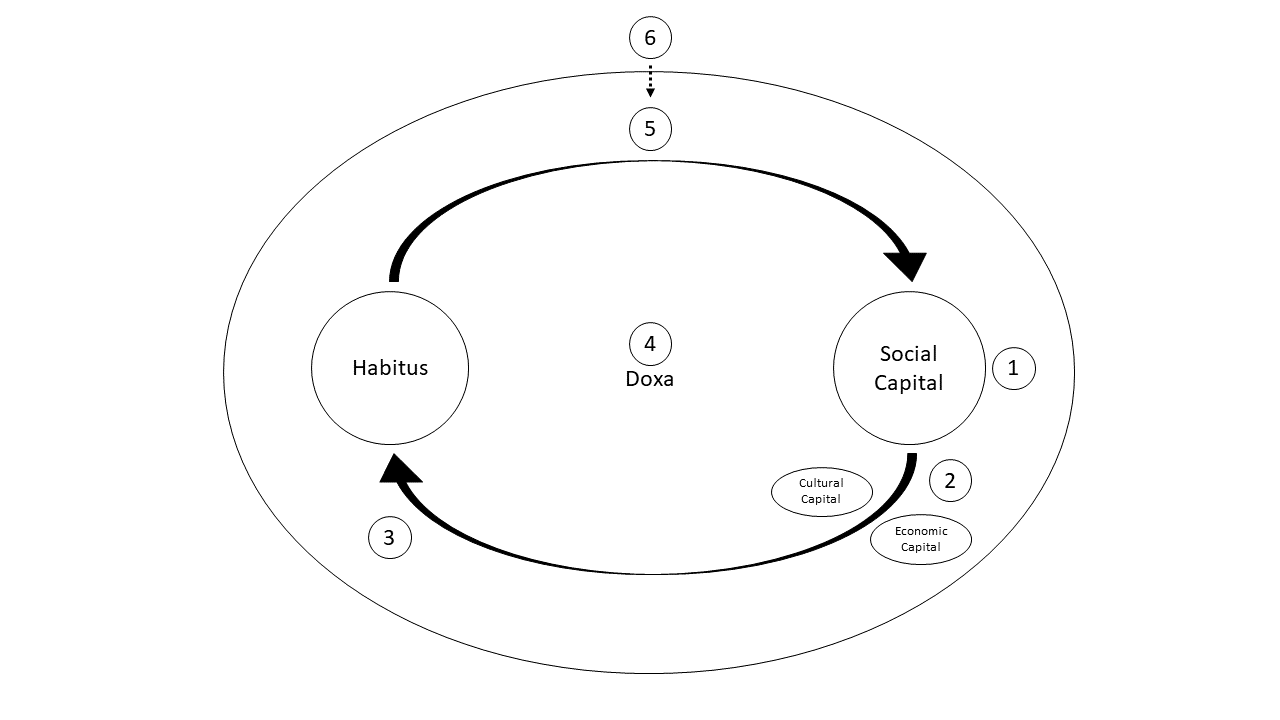
\includegraphics[width=\textwidth]{C5 - Understanding Capital Accumulation/HabitusSocCap_TheoreticalModel.png}
\caption{\label{fig:TheoreticalModel_C5}\textbf{Complete Theoretical Model}. The complete theoretical model. The model, informed by the described experiences of university science students, expands on the interaction between habitus and capital originally illustrated by \cite{Bourdieu1984}. The model provides a step by step description of how social capital translates into habitus transformation, and how habitus generates future capital accumulation. Step 1 refers to the initial availability of social capital for an individual. Step 2 refers to the value gained through leveraging social capital into forms of economic and cultural capital. Step 3 refers to how social capital is internalised by the individual. Step 4 refers to how habitus informs the acquisition of future social capital. 5 refers to factors outside of the individual that structure the field (by availability of capital and exchange value).}
\end{figure}

\section{Social Capital in the Field of University Science (Step 1)}
This section discusses the availability of social relationships that participants had in the field of university science (Figure \ref{fig:TheoreticalModel1_C5}). These relationships are categorised into three key groups, social capital through family connections, social capital through lecturers, and social capital through peers. 

\begin{figure}[h!]
\centering
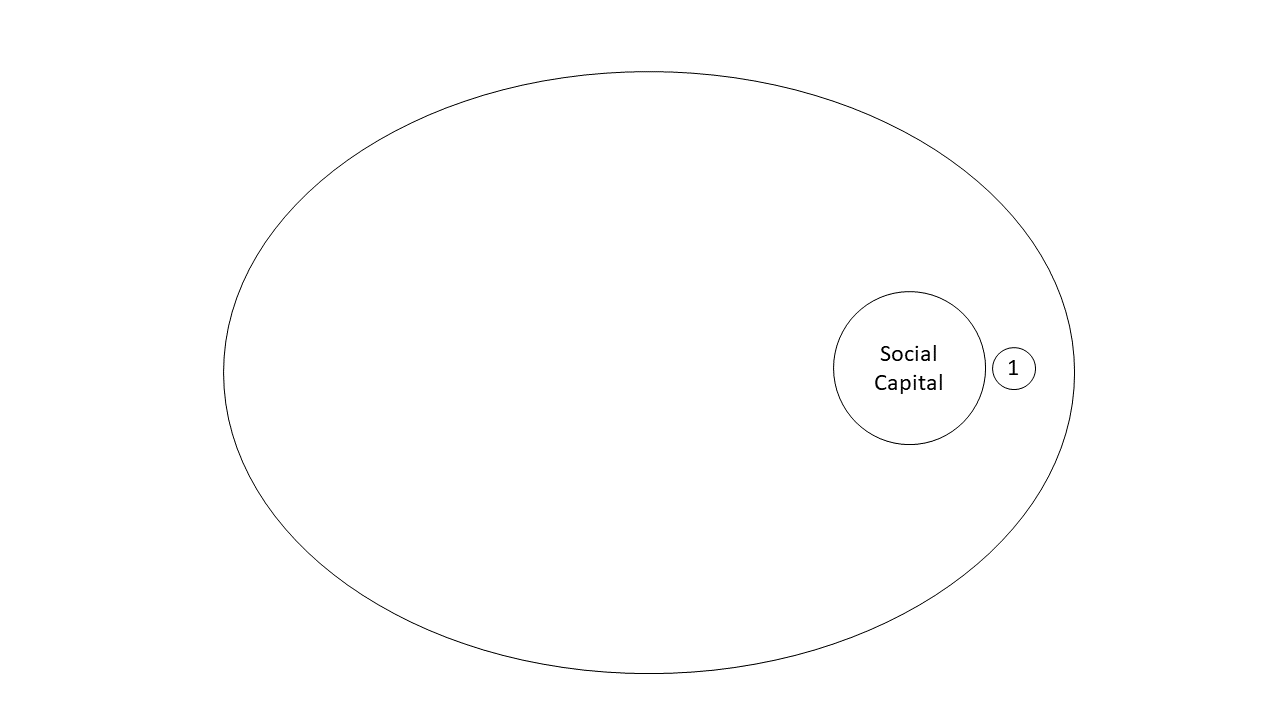
\includegraphics[width=\textwidth]{C5 - Understanding Capital Accumulation/HabitusSocCap_TheoreticalModel1.png}
\caption{\label{fig:TheoreticalModel1_C5}\textbf{Step 1}. The first step of the theoretical model. Step 1 refers to the initial availability of social capital for an individual.}
\end{figure}

The relationships that students share have been found to be important factors in success in university science. Research has shown that increasing access to mentors can improve outcomes for undergraduate students in the life sciences \citep{aikens2016social}. 


\section{Leveraging Social Capital (Step 2)}
The value of social capital is derived from the economic and cultural capital that can be mobilised through connections with others (Figure \ref{fig:TheoreticalModel2_C5}). These resources may provide students with advantages in supporting their learning and providing student access to information about the field. 

\begin{figure}[ht]
\centering
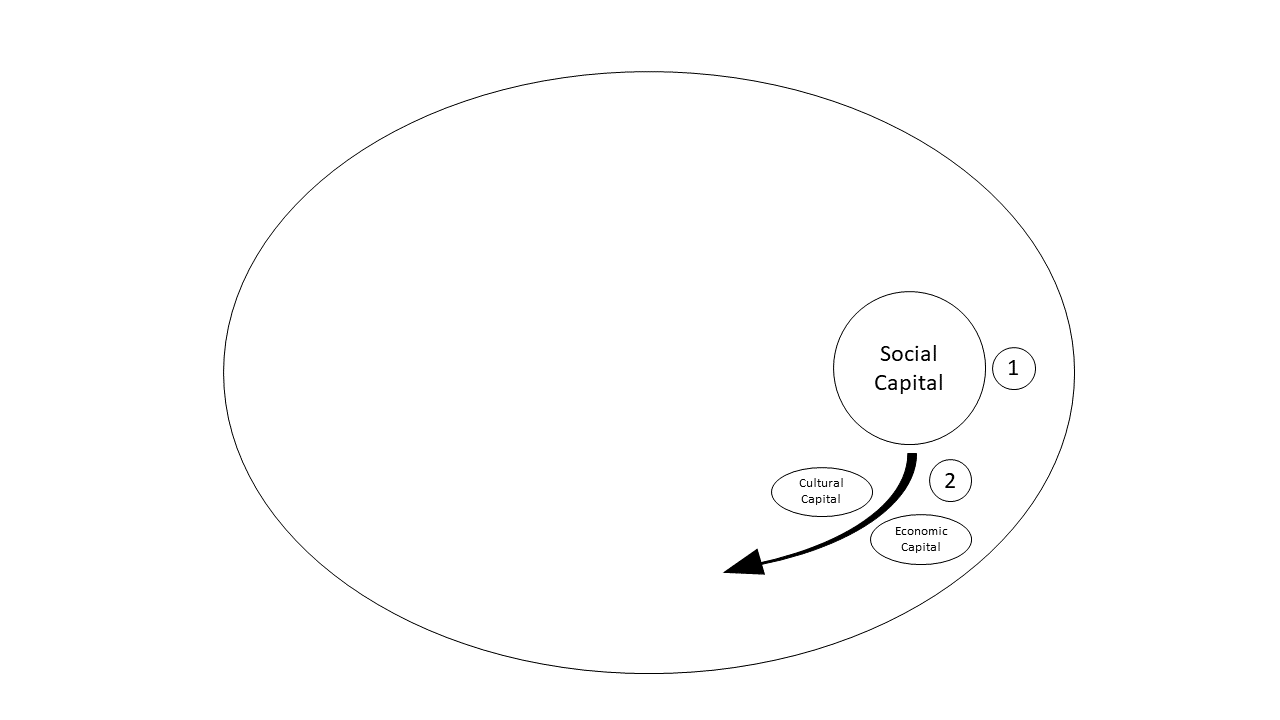
\includegraphics[width=\textwidth]{C5 - Understanding Capital Accumulation/HabitusSocCap_TheoreticalModel2.png}
\caption{\label{fig:TheoreticalModel2_C5}\textbf{Step 2}. The second step of the theoretical model. This step refers to the utility of social capital in mobilising cultural capital and economic capital.}
\end{figure}

Inequities in science education outcomes exist not only in the access individuals have to capital, but also in the value that society places on the capital that different groups hold. In the field of science, a wealth of research has shown that value is often defined by the terms of those who have historically held power in the field. Across gender, ethnicity, social class, sexual orientation, and disability, those who are less well-represented are more likely to feel out of place and marginalised. 


\section{Internalising Capital (Step 3)}
The capital that students accrue in university science not only provides access to resources, but it can also influences the way that students see themselves in the field. Capital, which determines students position in the field, is internalised by students via their habitus  (Figure \ref{fig:TheoreticalModel3_C5}), which establishes the students disposition towards the field \cite{Bourdieu1992}. Students who hold high levels of social capital may feel an affinity with the field and see progression to university as a path already drawn out.

The process of socialisation.
The process of objectified cultural capital transforming into embodied cultural capital (physical and mental - habitus)

\begin{figure}[ht]
\centering
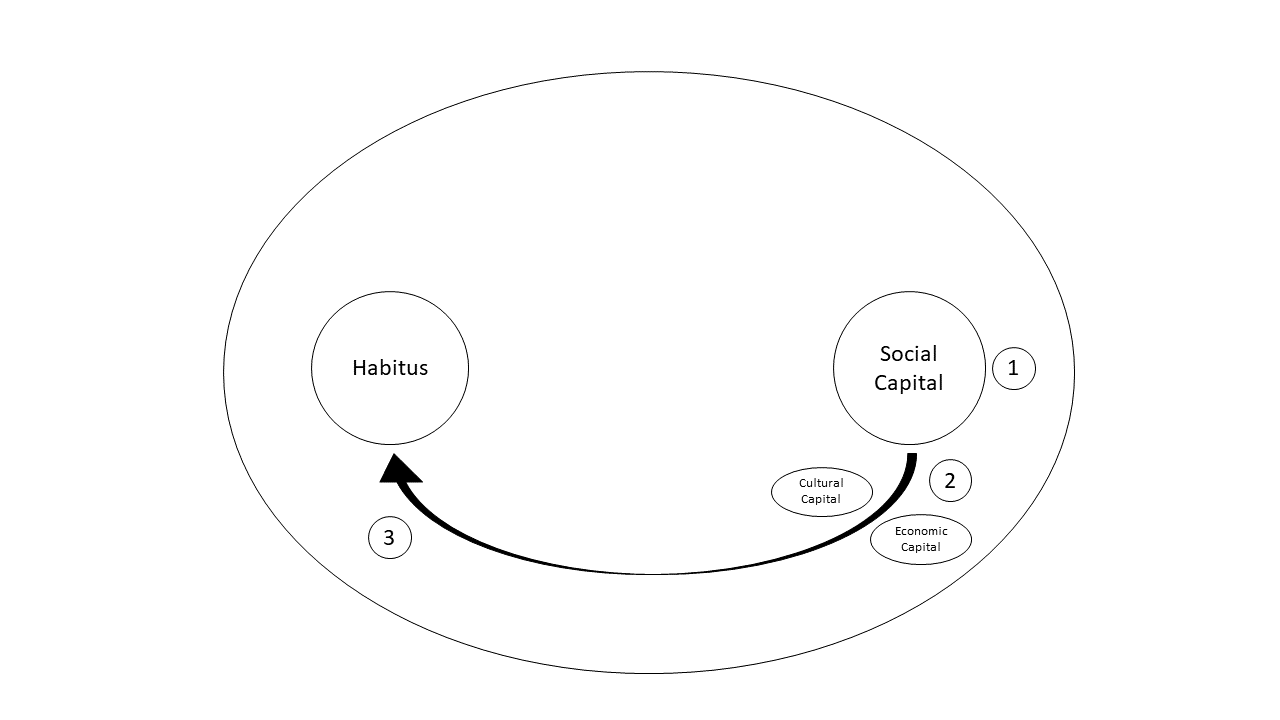
\includegraphics[width=\textwidth]{C5 - Understanding Capital Accumulation/HabitusSocCap_TheoreticalModel3.png}
\caption{\label{fig:TheoreticalModel3_C5}\textbf{Step 3}. The third step of the theoretical model. This step refers to the manner in which capital is internalised by individuals via habitus.}
\end{figure}



\section{Doxa (Step 4)}
Outside of the of the social relationships that students hold, general discourses in society influence the development of habitus (Figure \ref{fig:TheoreticalModel4_C5}). 

Bourdieu uses the term ``classed habitus'' to refer to the way in which members of the same social group are exposed to similar experiences and thus have similar dispositions and lifestyle practices. The concept of classed habitus has since been used in research in terms of gendered habitus \citep{Reay_2004}, Chinese habitus \citep{Mu2014}. Theorists advocating for intersectional approaches to identity research argue that experiences may be vastly different for individuals based on. For example, research shows that women of colour face many different barriers to success in the field of physics \cite{ong2005body}.

\begin{figure}[ht]
\centering
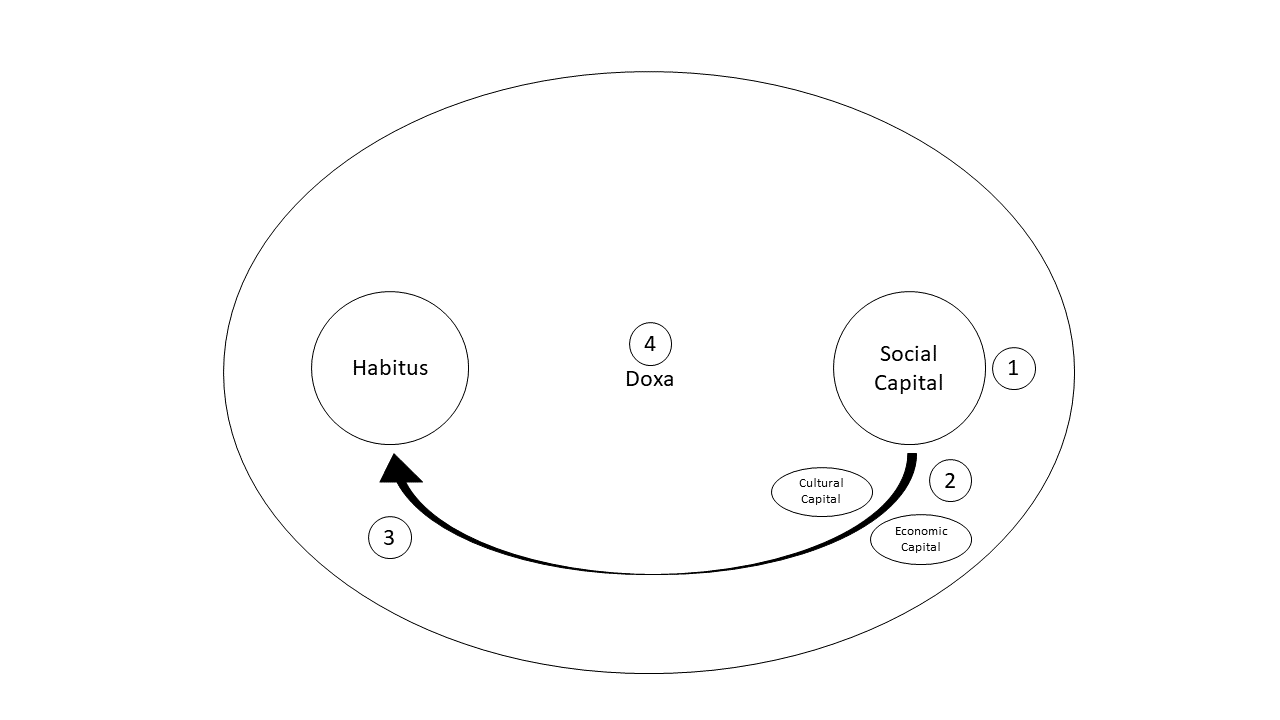
\includegraphics[width=\textwidth]{C5 - Understanding Capital Accumulation/HabitusSocCap_TheoreticalModel4.png}
\caption{\label{fig:TheoreticalModel4_C5}\textbf{Step 4}. The fourth step of the theoretical model. This step refers to the impact doxa (pervasive societal discourses) has on students' habitus.}
\end{figure}

\section{Generating Social Capital (Step 5)}
The future acquisition of social capital is informed by habitus (Figure \ref{fig:TheoreticalModel5_C5}). 

Students who lack capital entering into university may need to make sacrifices to other aspects of their life to get ahead. 

\begin{figure}[ht]
\centering
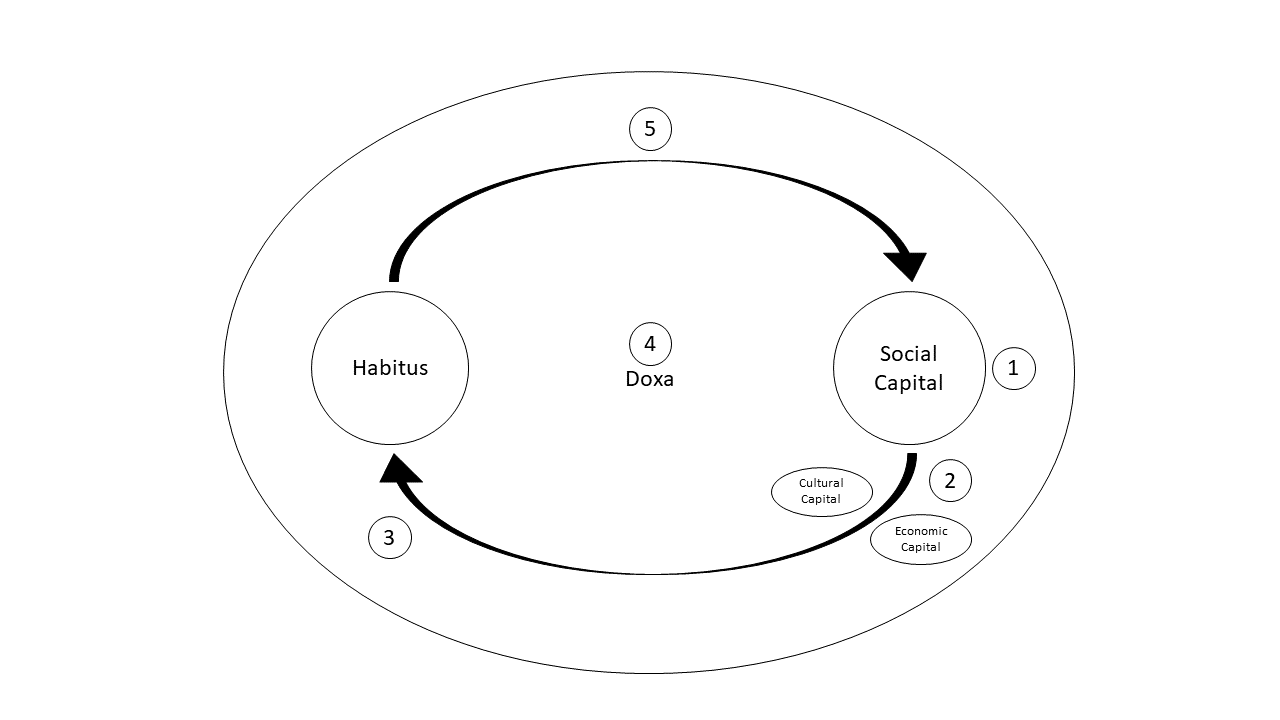
\includegraphics[width=\textwidth]{C5 - Understanding Capital Accumulation/HabitusSocCap_TheoreticalModel5.png}
\caption{\label{fig:TheoreticalModel5_C5}\textbf{Step 5}. The fifth step of the theoretical model. This step refers to the manner in which students' habitus directs the future acquisition of social capital}
\end{figure}



\section{Institutional Habitus (Step 6)}
The cycle is impacted on by interventions operating in the field, which themselves are directed by an institutional habitus (Figure \ref{fig:TheoreticalModel6_C5}). 

\begin{figure}[ht]
\centering
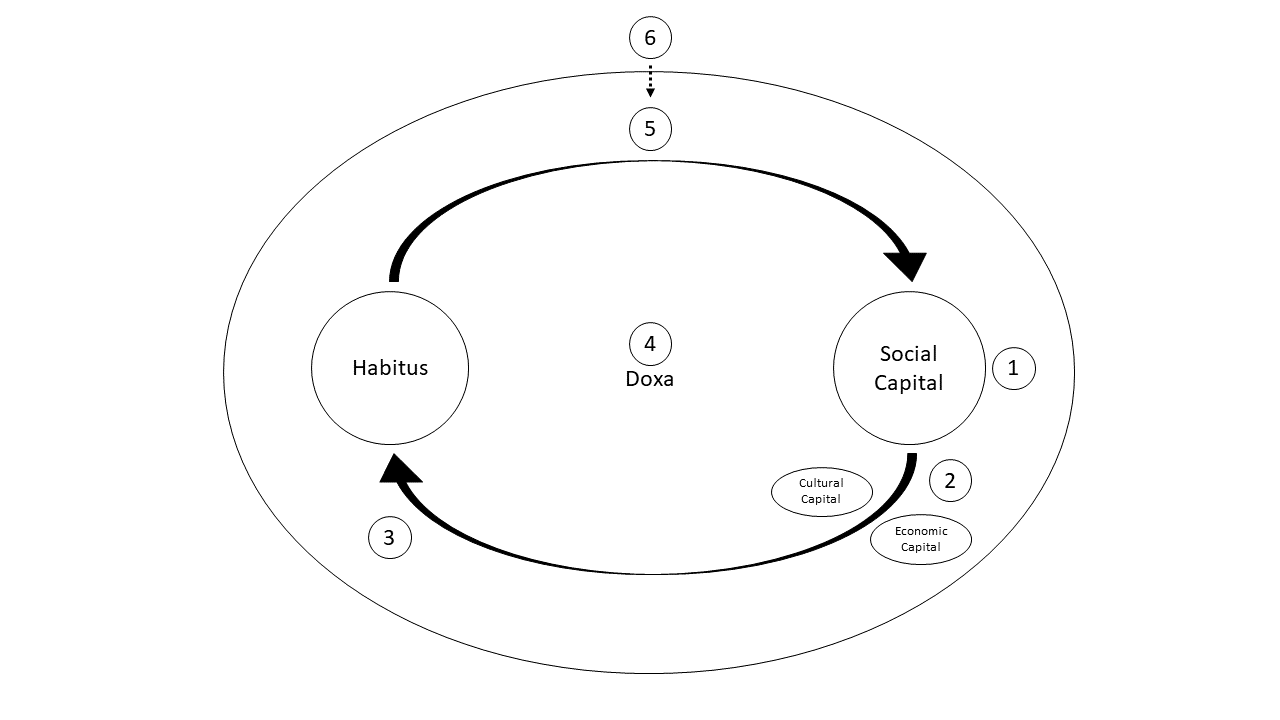
\includegraphics[width=\textwidth]{C5 - Understanding Capital Accumulation/HabitusSocCap_TheoreticalModel.png}
\caption{\label{fig:TheoreticalModel6_C5}\textbf{Step 6}. The sixth step of the theoretical model. This step refers to the manner in which institutions impact on the cycle}
\end{figure}



\section{Conclusion}


